\documentclass[letterpaper,10pt]{article}
\usepackage[margin=2cm]{geometry}

\usepackage{graphicx}
\usepackage{amsmath}
\usepackage{amsfonts}
\usepackage{amssymb}
\usepackage[colorlinks]{hyperref}
\usepackage{listings}

\newcommand{\panhline}{\begin{center}\rule{\textwidth}{1pt}\end{center}}

\title{\textbf{Linear Regression}}
\author{Aarti Singh (Instructor), HMW-Alexander (Noter)}

\begin{document}

\maketitle

\panhline
\href{../index.html}{Back to Index}

\panhline
\tableofcontents

\section*{Resources}

\begin{itemize}
	\item \href{../../Lectures/04_LinearRegression.pdf}{Lecture}
\end{itemize}

\panhline

\section{Discrete to Continuous Labels}
	
From classification to regression

\subsection{Task}

Given $X\in \mathcal{X}$, predict $Y \in \mathcal{Y}$, Construct prediction rule $f:\mathcal{X} \rightarrow \mathcal{Y}$

\subsection{Performance Measure}

\begin{itemize}
	\item Quantifies knowledge gained.
	\item Measure of closeness between true label Y and prediction f(X)
	\begin{itemize}
		\item 0/1 lose:$loss(Y,f(X))=1_{f(X)\neq Y}$. Risk: probability of error 
		\item square loss: $loss(Y,f(X))=(f(X)-Y)^2$. Risk: mean square error
	\end{itemize}
	\item How well does the predictor perform on average?
	$$Risk~R(f)=\mathbb{E}[loss(Y,f(X))],~(X,Y)\sim P_{XY}$$
\end{itemize}

\subsection{Bayes Optimal Rule}

\begin{itemize}
	\item ideal goal: Construct prediction rule $f^*:\mathcal{X}\rightarrow\mathcal{Y}$
	$$f^*=\arg\min_f{E_{XY}[loss(Y,f(X))]}$$ (Bayes optimal rule)
	\item Best possible performance:
	$$\forall f,~R(f^*) \leq R(f)$$ (Bayes Risk)
\end{itemize}

Problem: $P_{XY}$ is unknown.

Solution: Training data provides a glimpse of $P_{XY}$
$$\text{(observed)~}\{(X_i,Y_i)\} \sim_{i.i.d} P_{XY}\text{~unknown}$$

\section{Macine Learning Algortihm}

\begin{itemize}
	\item Model based approach: use data to learn a model for $P_{XY}$
	\item Model-free approach: use data to learn mapping directly
\end{itemize}

\subsection{Empirical Risk Minimization (model-free)}

\begin{itemize}
	\item Optimal predictor: $$f^*=\arg\min_f{\mathbb{E}[(f(X)-Y)^2]}$$
	\item Empirical Minimizer: $$\hat{f}_n=\arg\min_{f\in\mathcal{F}}\frac{1}{n}\sum_{i=1}^{n}(f(X)-Y)^2$$
\end{itemize}

$\mathcal{F}$ is the class of predictors:
\begin{itemize}
	\item Linear
	\item Polynomial
	\item Nonlinear
\end{itemize}

\section{Linear Regression}

$$f(\vec{X})=\sum_{i=0}^{p}{\beta_0X^{i}}=\vec{X}^T\vec{\beta},~where~X^0=1,~\vec{\beta}=[\beta_0,\dots,\beta_p]^T$$

$$\hat{\vec{\beta}}=\arg\min_{\vec{\beta}}(A^T\vec{\beta}-\vec{Y})^T(A^T\vec{\beta}-\vec{Y}),~where~A=[\vec{X_1},\dots,\vec{X_n}]$$

$$J(\beta)=(A^T\vec{\beta}-\vec{Y})^T(A^T\vec{\beta}-\vec{Y})$$

\begin{equation*}
\begin{array}{rcl}
\frac{\partial J(\vec{\beta})}{\partial \vec{\beta}} & = & \frac{\partial (A^T\vec{\beta}-\vec{Y})^T(A^T\vec{\beta}-\vec{Y})}{\partial \vec{\beta}} \\
& = & \frac{\partial (\vec{\beta}^TAA^T\vec{\beta}-\vec{\beta}^TA\vec{Y}-\vec{Y}^TA^T\vec{\beta}+\vec{Y}^T\vec{Y})}{\vec{\beta}} \\
& = & (AA^T+(AA^T)^T)\vec{\beta}-A\vec{Y}-A\vec{Y} \\
& = & 2AA^T\vec{\beta}-2A\vec{Y} = 0 \\
& \Rightarrow & AA^T\vec{\beta}=A\vec{Y} \\
& \Rightarrow & \hat{\vec{\beta}}=(AA^T)^{-1}A\vec{Y},~\text{if $AA^T$ is invertible}
\end{array}
\end{equation*}

\subsection{Gradient Descent}

Even when $AA^T$ is invertible, might be computationally expensive if $A$ is huge; however, $J(\vec{\beta})$ is convex\footnote{A function is called convex if the line joining any two points on the function does not go below the function on the interval formed by these two points.} in $\beta$.

Minimum of a convex function can be reached by gradient descent algorithm:
\begin{itemize}
	\item Initialize: pick $\vec{w}$ at random
	\item Gradient: $$\nabla_{\vec{w}} l(\vec{w})=[\frac{\partial l(\vec{w})}{\partial w_0},\dots,\frac{\partial l(\vec{w})}{\partial w_d}]^T$$
	\item Update rule: $$\Delta \vec{w}=\eta \nabla_{\vec{w}}l(\vec{w})$$, $$w_i^{t+1} \leftarrow w_i^t - \eta \frac{\partial l(\vec{w})}{\partial w_i}|_t$$
	\item Stop: when some criterion met $\frac{\partial l(\vec{w})}{\partial w_i}|_t < \epsilon$
\end{itemize}



\subsection{If $AA^T$ is not invertible}

$Rank(AA^T)$ = number of non-zero eigenvalues of $AA^T$ = number of non-zero singular values of A $\leq \min(n,p)$ since $A$ is $n\times p$

$$A=U \Sigma V^T \Rightarrow AA^T=U\Sigma^2U^T \Rightarrow AA^T U = U\Sigma^2$$

\subsubsection{Regularized Leasts Squares}

Ridge Regression (L2 penalty)

\begin{equation}
\begin{array}{rcl}
\hat{\vec{\beta}}_{MAP} & = & \arg\min_{\vec{\beta}}(A^T\vec{\beta}-\vec{Y})^T(A^T\vec{\beta}-\vec{Y}) +\lambda \vec{\beta}^T\vec{\beta}~~(\lambda \geq 0) \\
& = & (AA^T + \lambda I)^{-1} A\vec{Y}
\end{array}
\end{equation}

$(AA^T + \lambda I)$ is invertible if $\lambda > 0$. Proof:
\begin{itemize}
	\item the symmetric matrix $AA^T$ is positive-semidefinite matrix, because a matrix is positive-semidefinite iff it arises as the Gram matrix of some set of vectors\footnote{In contrast to the positive-definite case, these vectors need not be linearly independent.}.
	\item $\therefore \forall \lambda>0~and~\vec{x}\neq\vec{0}$, 
	$$\vec{x}^T(AA^T)\vec{x} = (A^T\vec{x})^T(A^T\vec{x}) \geq 0$$
	$$\vec{x}^T(AA^T+\lambda I)\vec{x} = \vec{x}^T (AA^T) \vec{x} + \lambda \vec{x}^T\vec{x} >0$$
	\item $\therefore$ $(AA^T+\lambda I)$ is positive definite.
	\item $\therefore$ the eigenvalues of $B=(AA^T+\lambda I)$ are all positive. $$B\vec{v}=\lambda\vec{v} \Rightarrow \vec{v}^T B \vec{v} = \lambda >0$$
	\item $\therefore$ $(AA^T + \lambda I)$ is invertible if $\lambda > 0$
\end{itemize}

\subsubsection{Understanding Regularized Least Squared}

Why we need constraints: r equations, p unknowns - underdetermined system of linear equations. 

$$\min_{\vec{\beta}} J(\beta)+\lambda pen(\vec{\lambda})$$
\begin{itemize}
	\item Ridge Regression: $pen(\beta)=||\beta||_2^2$
	\item Lasso Regression: $pen(\beta)=||\beta||_1$. No closed form solution, but can optimize using sub-gradient descent.
	\item $pen(\beta)=||\beta||_0=\sum 1_{\beta_i \neq 0}$
\end{itemize}

\begin{figure}[!h]
	\centering
	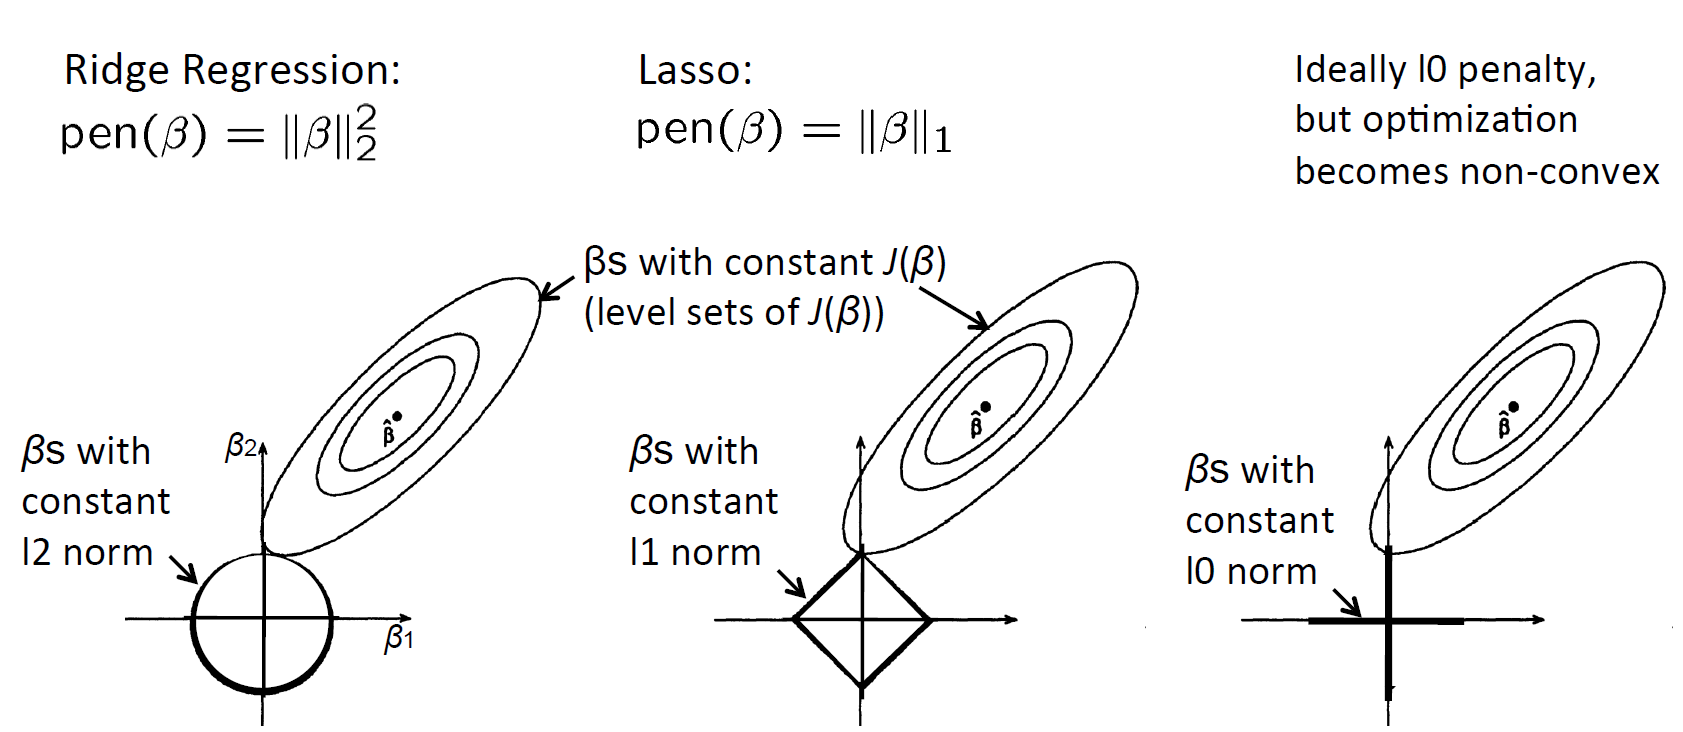
\includegraphics[width=10cm]{./img/ridgeregression.png}
	\caption{For Lasso regression, results are in sparse solution - vector with more zero coordinates. Good for high-dimenstional problems - don't have to store all coordinates, interpretable solution! }
\end{figure}

Matlab code:
\begin{lstlisting}[language=Matlab]
[B,FitInfo] = lasso(X,Y,Name,Value)
\end{lstlisting}
\begin{itemize}
	\item X: Numeric matrix with n rows and p columns. Each row represents one observation, and each column represents one predictor (variable).
	\item Y: Numeric vector of length n, where n is the number of rows of X. Y(i) is the response to row i of X.
	\item 'Alpha': Scalar value from 0 to 1 (excluding 0) representing the weight of lasso (L1) versus ridge (L2) optimization. Alpha = 1 represents lasso regression, Alpha close to 0 approaches ridge regression, and other values represent elastic net optimization. See Definitions.
	Default: 1
\end{itemize}



\subsection{Regularized Least Squares - Connection to MLE and MAP (Model-based Approaches)}

\subsubsection{Least Squares and M(C)LE (Maximum Conditional Likelihood Estimator)}

$$Y=f^*(X)+\epsilon=X\beta^*+\epsilon$$
$$\epsilon \sim \mathcal{N}(0,\sigma^2I)~~Y\sim\mathcal{N}(X\beta^*,\sigma^2I)$$
$$\hat{\beta}_{MLE} = \arg\max_\beta (\log p(\{Y_i\}|\beta,\sigma^2,\{X_i\}))=\arg\min_{\beta}\sum_i(X_i\beta-Y_i)^2$$
\begin{itemize}
	\item Model parameters: $\beta,\sigma^2$
	\item Conditional log likelihood: $\log p(\{Y_i\}|\beta,\sigma^2,\{X_i\})$
\end{itemize}

Least Square Estimator is same as Maximum Conditional Likelihood Estimator under a Gaussian model.

\subsubsection{Regularized Least Squares and M(C)AP (Maximum Conditional A Prior Estimator)}

If $AA^T$ is not invertible.

$$Y=f^*(X)+\epsilon=X\beta^*+\epsilon$$
$$\epsilon \sim \mathcal{N}(0,\sigma^2I)~~Y\sim\mathcal{N}(X\beta^*,\sigma^2I)$$
(1) Gaussian prior:
$$\beta \sim \mathcal{N}(0,\tau^2 I)~~p(\beta) \propto \exp(-\beta^T\beta/2\tau^2)$$
$$\hat{\beta}_{MAP} = \arg\max_\beta \log p(\{Y_i\}|\beta,\sigma^2,\{X_i\}) +\log p(\beta)=\arg\min_{\beta}\sum_i(X_i\beta-Y_i)^2+\lambda(\sigma^2,\tau^2)||\beta||_2^2$$
(2) Laplace prior:
$$\beta \sim Laplace(0,t)~~p(\beta_i) \propto \exp(-|\beta_i|/t)$$
$$\hat{\beta}_{MAP} = \arg\max_\beta \log p(\{Y_i\}|\beta,\sigma^2,\{X_i\}) +\log p(\beta)=\arg\min_{\beta}\sum_i(X_i\beta-Y_i)^2+\lambda(\sigma^2,\tau^2)||\beta||_1$$


\begin{itemize}
	\item Model parameters: $\beta,\sigma^2$
	\item Conditional log likelihood: $\log p(\{Y_i\}|\beta,\sigma^2,\{X_i\})$
	\item Log prior: $\log p(\beta)$
\end{itemize}

\section{Polynomial Regression}

\begin{itemize}
	\item Univariate: $f(X)=\sum{\beta_iX^i}=[1, X, X^2, \dots, X^m]^T\beta$
	$$\hat{\beta}=(AA^T)^{-1}AY~or~(AA^T+\lambda I)^{-1}AY$$
	\item Multivariate: $f(X) = \sum_i{\beta_i X^{(i)}} + \sum_{i,j}{\beta_{i,j} X^{(i)} X^{(j)}}+\sum_{i,j,k}{\beta_{i,j,k} X^{(i)} X^{(j)}X^{(k)}}+\dots$
\end{itemize}


\subsection{Bias - Vairance Tradeoff}
\begin{itemize}
	\item Large bias, small variance: poor approximation but robust/stable
	\item Small bias, large variance: good approximation but unstable
\end{itemize}

Bias-Variance Decomposition:
$$E[(f(X)-f^*(X))^2] = Bias^2 + Variance$$
\begin{itemize}
	\item $Bias = E[f(X)] - f^*(X)$: How far is the model from best model.
	\item $Variance = E[(f(X)-E[f(X)])^2]$: How variable is the model.
\end{itemize}

\begin{figure}[!h]
	\centering
	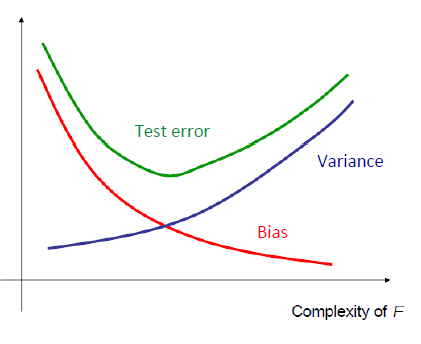
\includegraphics[width=8cm]{./img/testerror.png}
	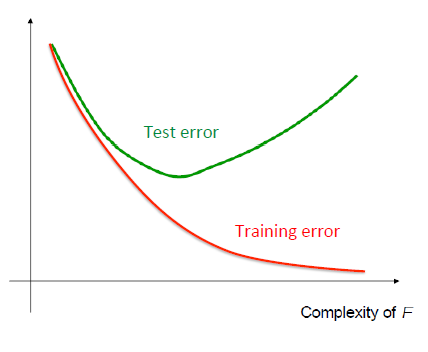
\includegraphics[width=8cm]{./img/trainerror.png}
\end{figure}

\section{Regression with Basis Functions or Nonlinear Features}

$$f(X)=\sum_i \beta_i \phi_i(X)$$


\end{document}



